
\section{Team PML 30 ${\varphi}$} 
		Team PML 30 ${\varphi}$ was assembled in September 2014 in the Russian city of St. Petersburg from 3 novices and one participant with experience, who was made captain. Tasks and roles were distributed among the participants, and we established safety rules. In the first place the team put spreading principles of honorable professionalism to others. All decisions were made collectively inside team with discussion to find the most optimal solutions. 
		During the year we took part in many events and everywhere we have tried to attract attention to our team and encourage people to take part in FTC. Also we pursued and distributed the principles of honorable professionalism. Talking to the press, we hoped to attract more attention to our team and to the competition in general, as well as attracting sponsors. The latter was important because of the need for funds - purchasing materials and equipment costs a lot.
		The team took part in the three qualifying competitions and in the regional finals. In all of them we made new contacts, shared experience and provided mutual assistance to other teams. In the first qualifying rounds in Sochi we met Stuy Fission 310 from USA and maintain contact with them to this day. On regional finals, we met with a team from Romania, Auto Vortex, and keep in touch with them through Facebook. Also, there is an active group chat with a large number of Russian teams. You can find the team page in Facebook at the address https://www.facebook.com/pages/FTC-team-PML30-PHI.
	    To increase the efficiency of our team work we used the version control system GitHub, which allows the entire team to work simultaneously on a single projects without losing files and providing easy way to resolve roblems. Also for writing technical books we been used professional typesetting system LaTeX.
	    \center{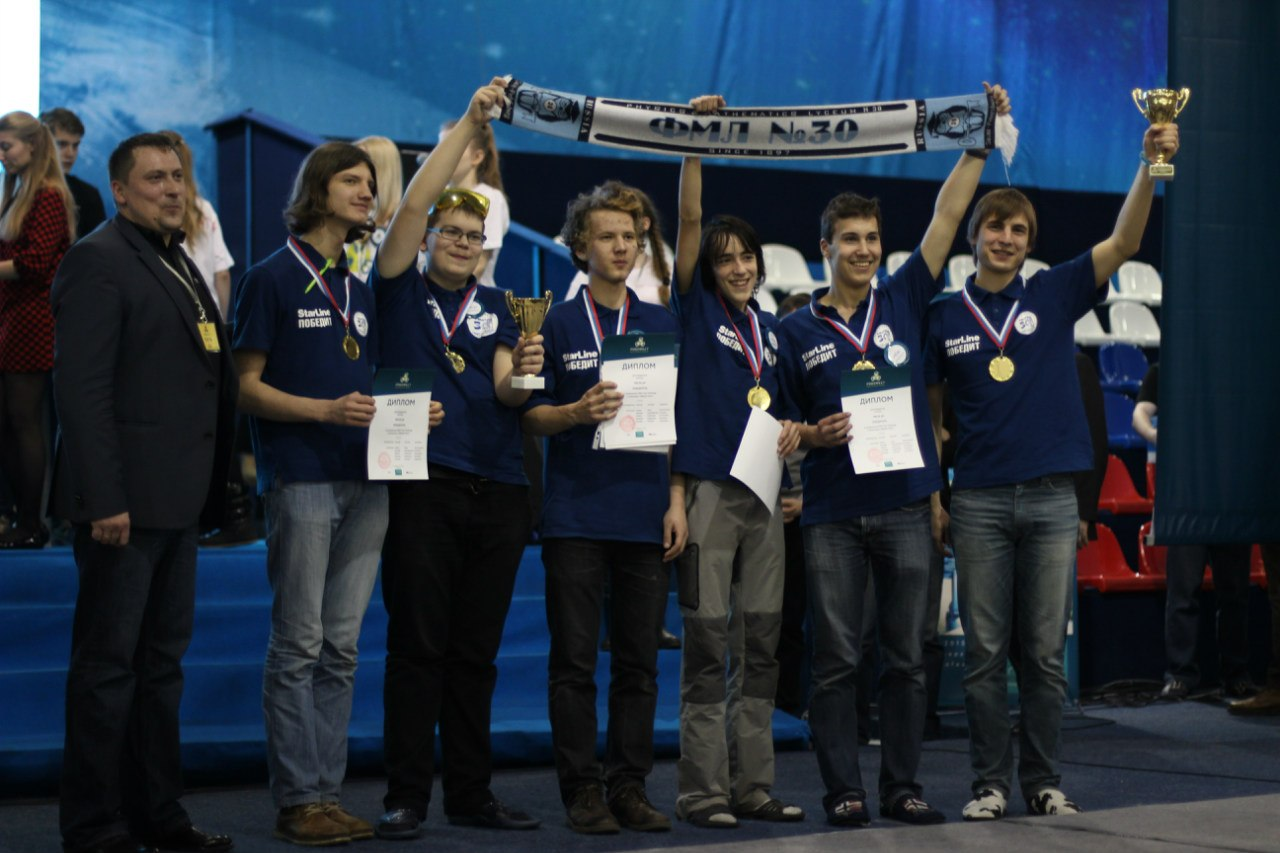
\includegraphics[scale=0.2]{days/Team/images/09}}\\
\begin{figure}[H]
	\begin{minipage}[h]{0.47\linewidth}
		\center{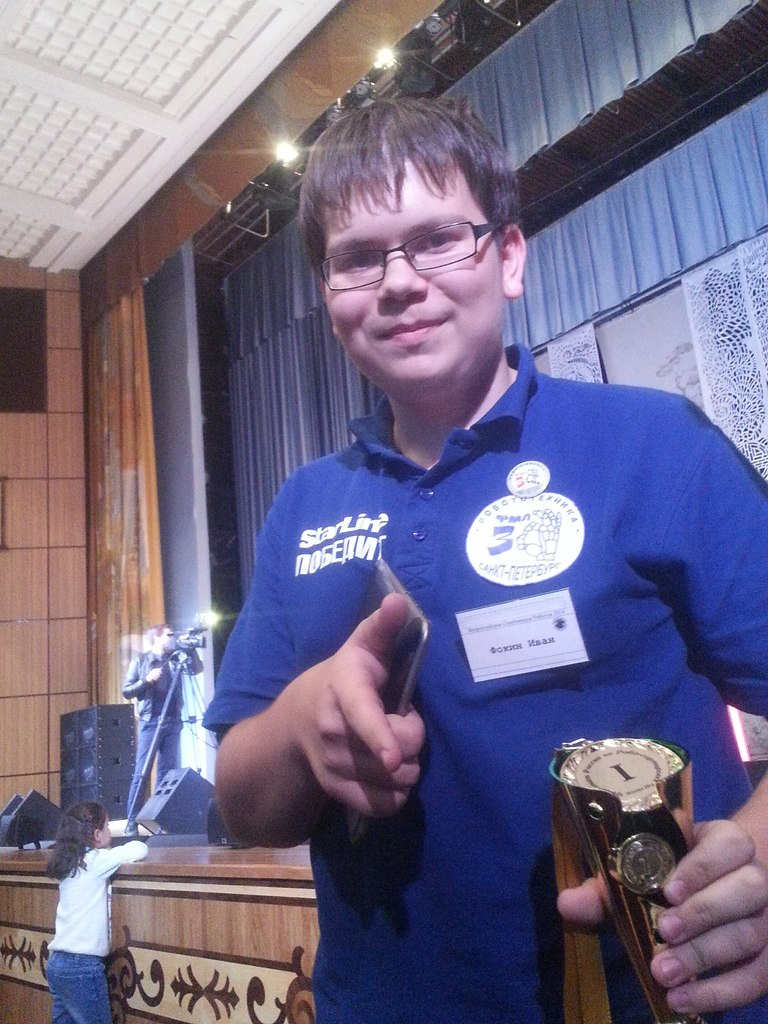
\includegraphics[scale=0.2]{days/Team/images/01}}\\
		Fokin Ivan\\
		\emph{Role in team: Captain, purchase of materials, strategy development in the game, communication with press, reserve  manipulator }
		\emph{Information: 17 years old, in robotics 5 years, in FTC 3 years } 
		\emph{Why I chose FTC: When I first I attended the event FTC saw hefty metal robots, with enthusiasm and without hesitation decided that I would like to do this.}
	\end{minipage}
	\hfill
	\begin{minipage}[h]{0.47\linewidth}
		\center{
\includegraphics[scale=0.25]{days/Team/images/02}}\\
		Radionov Maxim\\
		\emph{Role in team: communication with the team and community, decorating robot, power design, reserve operator}
		\emph{Information: 16 years old, in robotics 3 years, in FTC 1 years}
	\end{minipage}
	\center  
	\center  
	\vfill 
	\begin{minipage}[h]{0.47\linewidth}
		\center{
\includegraphics[scale=0.25]{days/Team/images/03}}\\
		Safronov Nikita\\
		\emph{Role in team: manipulator-1,  creation of 3D models, chief engineer, responsible for the robot assembly}
		\emph{Information: 16 years old, in robotics 3 years, in FTC 1 years} 
		\emph{Why I chose FTC: I have chosen FIRST because I enjoy working with mechanisms and finding unusual technical decisions for solving problems. Also working on this project helps me to get new skills in a sphere of engineering. In this case I know, that I don,t spend my time in vain.}			
	\end{minipage}
	\hfill
	\begin{minipage}[h]{0.47\linewidth}
		\center{
\includegraphics[scale=0.25]{days/Team/images/04}}\\
		Maksimychev Evgeniy\\
		\emph{Role in team: manipulator-2, responsible for accident prevention, responsible for technical book}
		\emph{Information: 15 years old, in robotics 2 years, in FTC 1 years}
		\emph{Why I chose FTC: "This is an interesting project that allows to implement some innovative solutions. In addition to the skills of designing robots, we also obtain the skills of the technical documentation and communication with colleagues which makes this competition as close to real engineering problems."}
	\end{minipage}
	\begin{minipage}[h]{0.47\linewidth}
		\center{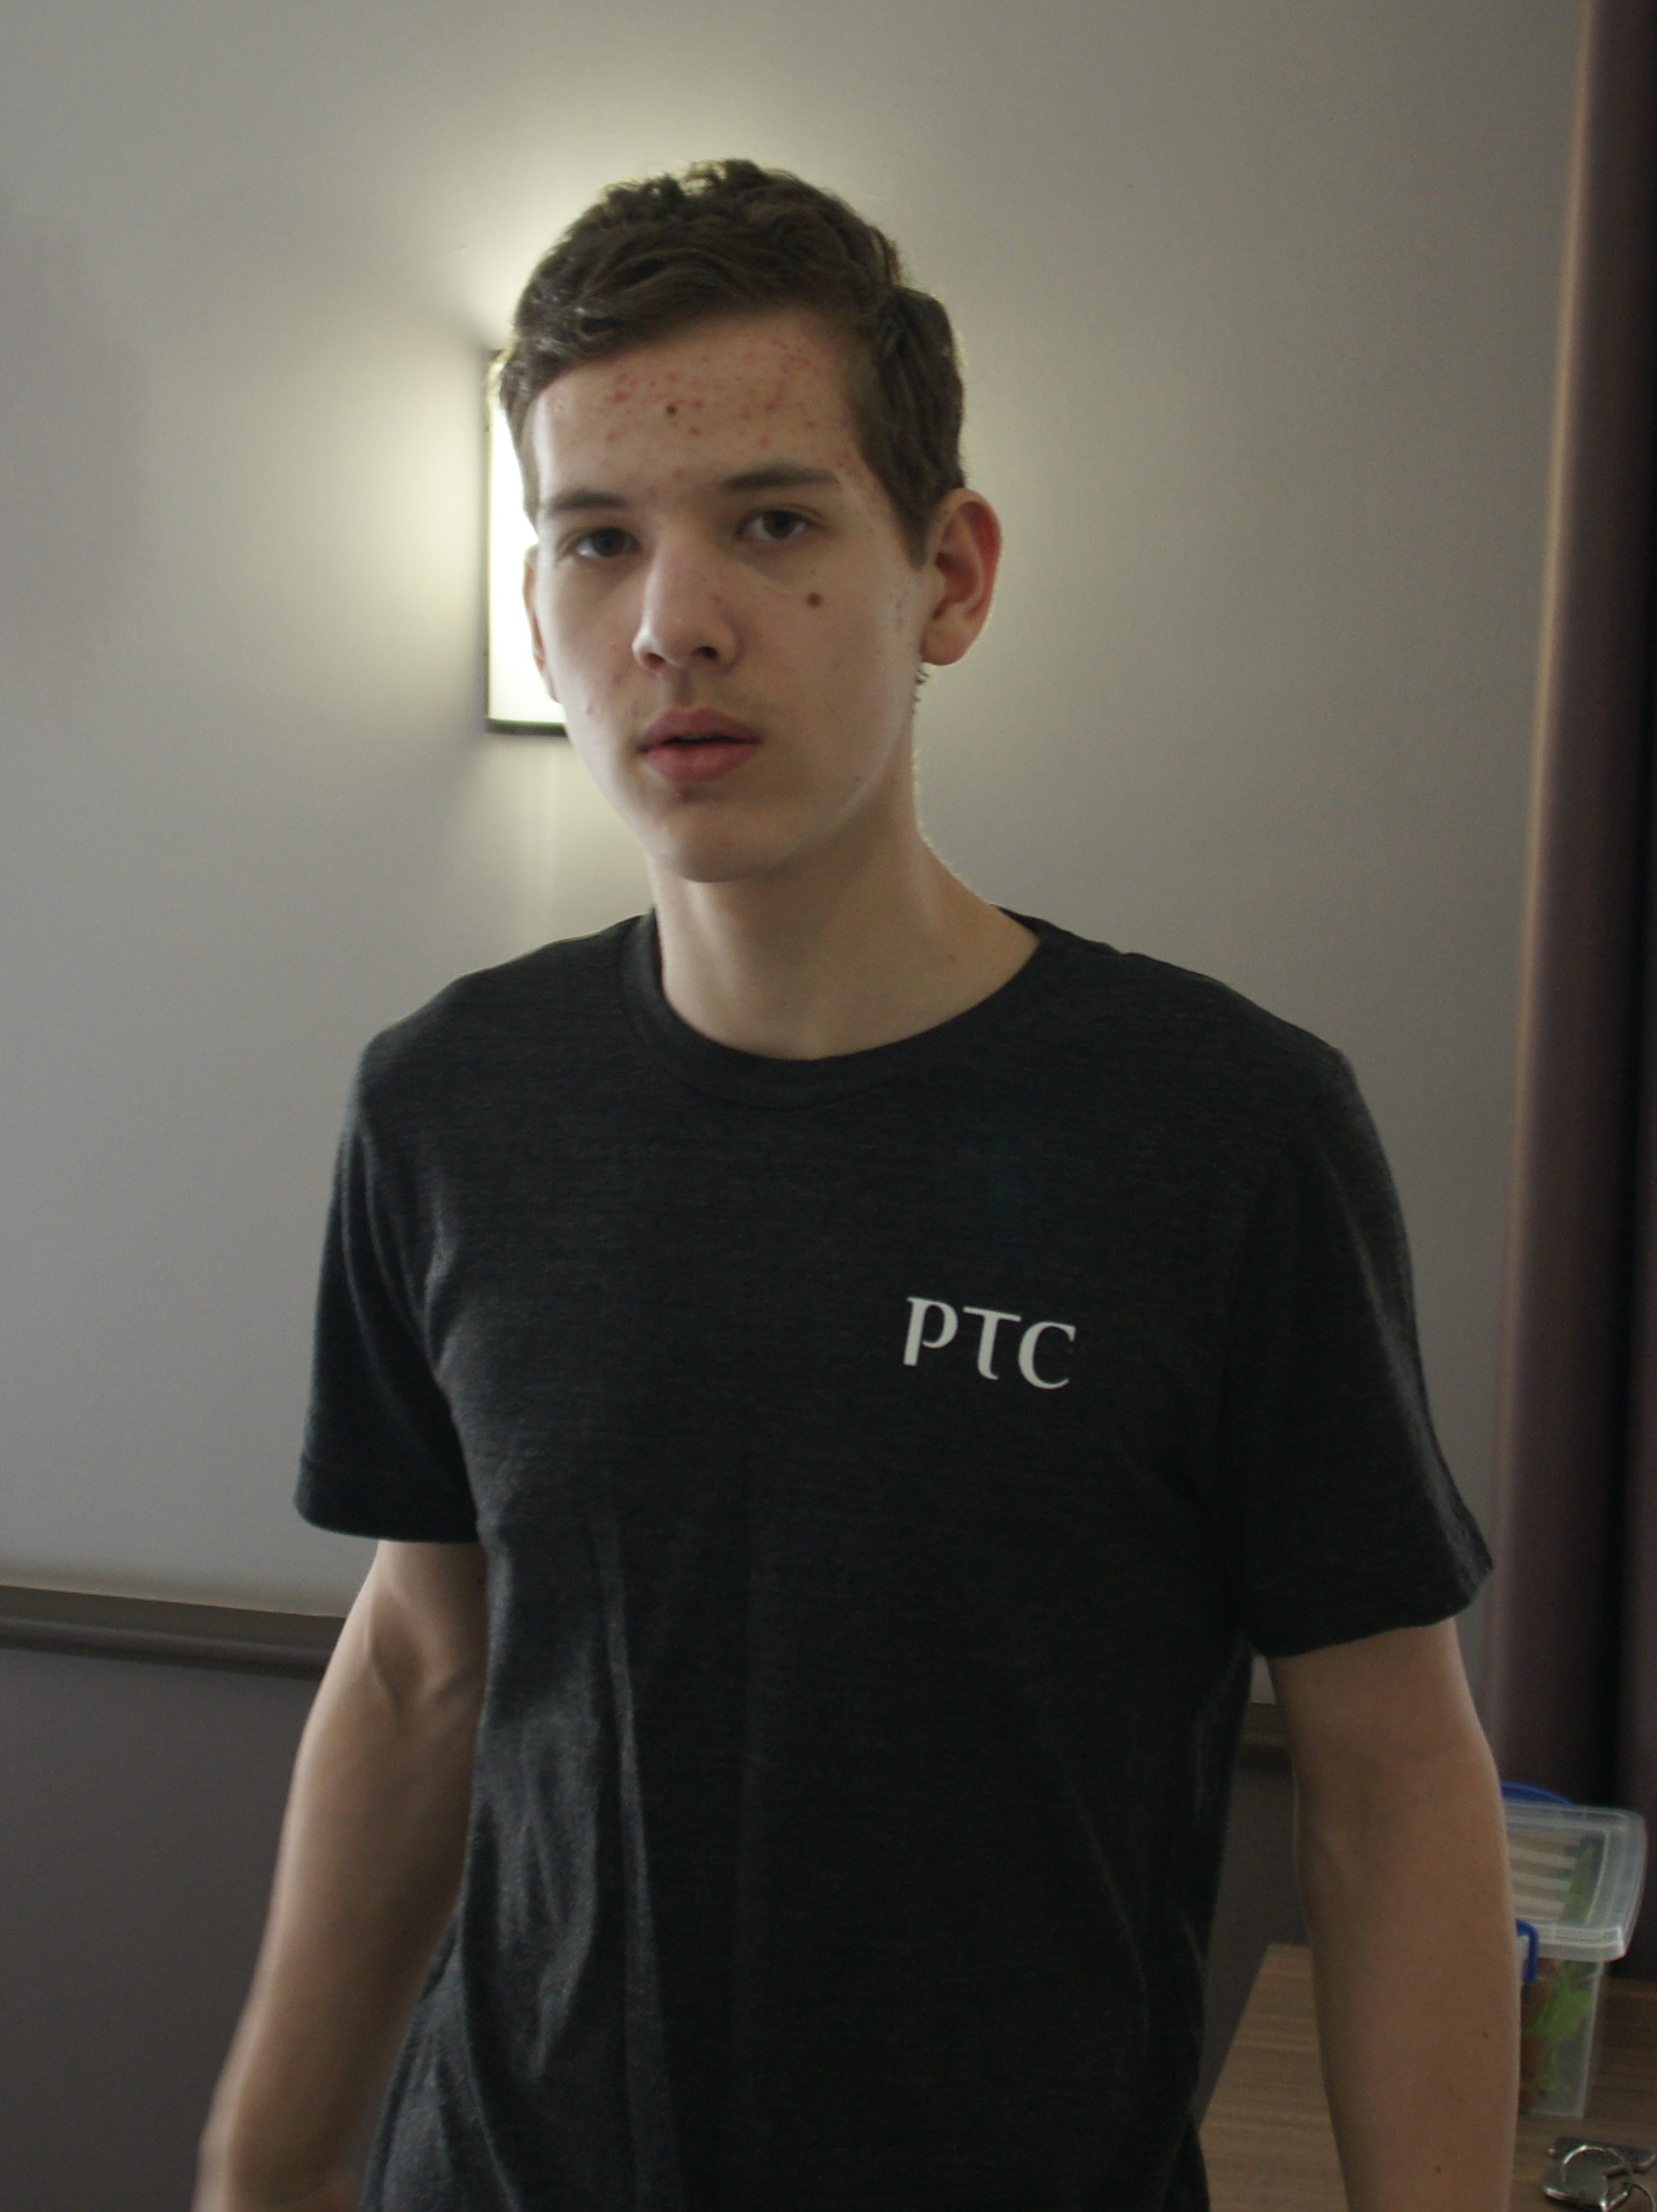
\includegraphics[scale=0.12]{days/Team/images/06}}\\
		\emph{Krylov Georguy}
			\emph{Role in team: coordinator of the action operators in game, responsible for robot modification.}
			\emph{Information: 17 years old, in robotics 3 years, in FTC 3 years }
				\emph{Why I chose FTC: "I chose the FTC because I like to come up with the design of robots and turn their ideas into reality, because every time I feel like a Creator who made a new creature."}
	\end{minipage}
\end{figure}

\newpage

\large  Instructors:

\begin{figure}[H]
	\begin{minipage}[h]{0.47\linewidth}
		\center{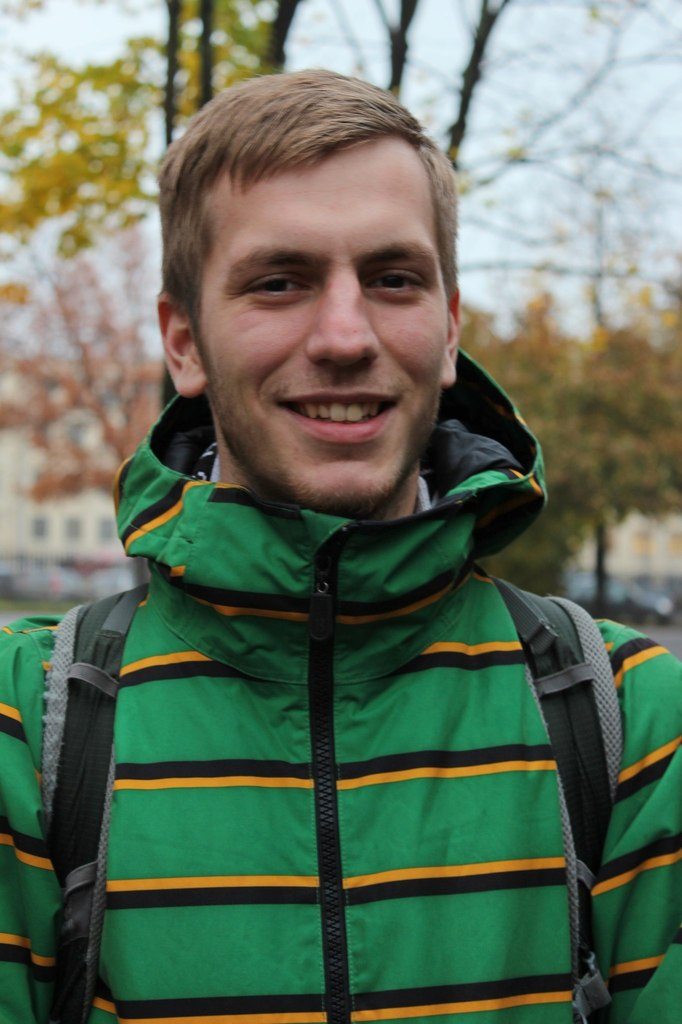
\includegraphics[scale=0.25]{days/Team/images/05}}\\
		\emph{Fedotov Anton} 
	\end{minipage}
	\hfill	
	\center  
	\center  
	\vfill 
	\begin{minipage}[h]{0.47\linewidth}
		\center{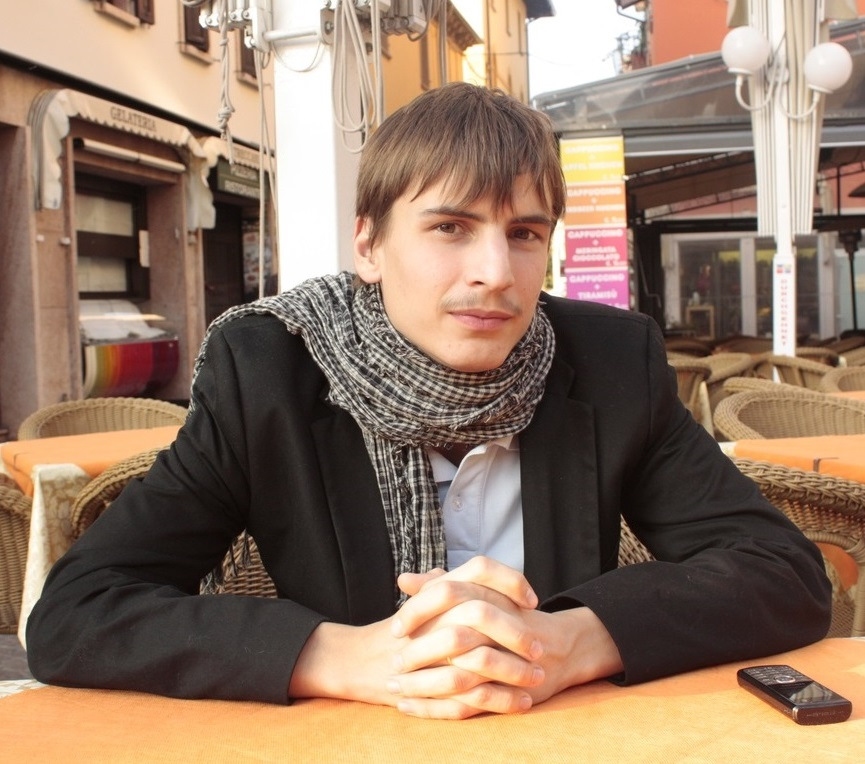
\includegraphics[scale=0.3]{days/Team/images/07}}\\
		\emph{Luzin Dmitruy}
	\end{minipage}
	\hfill
	\begin{minipage}[h]{0.47\linewidth}
		\center{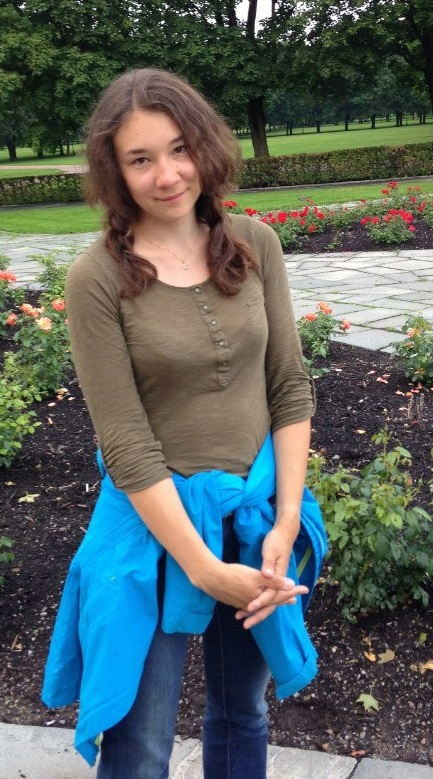
\includegraphics[scale=0.35]{days/Team/images/08}}\\
		\emph{Luzina Kate}
	\end{minipage}
\end{figure}

\newpage
